\definecolor{acmBlue}{HTML}{1F77B4}
\definecolor{acmTeal}{HTML}{009E73}
\definecolor{acmSand}{HTML}{D55E00}
\definecolor{acmGray}{HTML}{8A8F99}
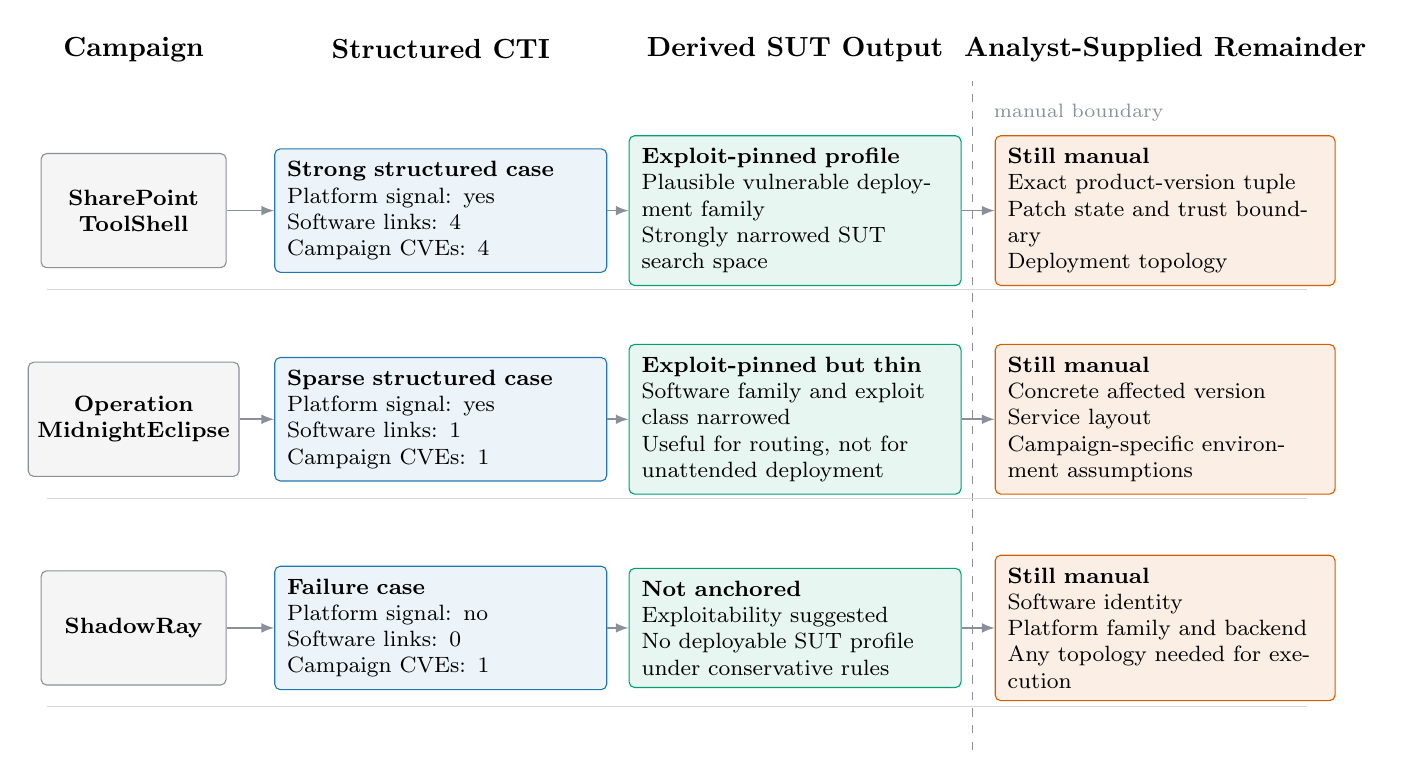
\begin{tikzpicture}[x=1cm,y=1cm,font=\footnotesize,>=latex]
  \node[font=\bfseries] at (1.55,9.25) {Campaign};
  \node[font=\bfseries] at (5.45,9.25) {Structured CTI};
  \node[font=\bfseries] at (9.95,9.25) {Derived SUT Output};
  \node[font=\bfseries] at (14.65,9.25) {Analyst-Supplied Remainder};

  \draw[dashed,acmGray,line width=0.5pt] (12.2,0.35) -- (12.2,8.85);
  \node[anchor=west,text=acmGray,font=\scriptsize] at (12.35,8.45) {manual boundary};

  \foreach \y in {7.2,4.55,1.9} {
    \draw[acmGray!35,line width=0.35pt] (0.45,\y-1.0) -- (16.45,\y-1.0);
  }

  % SharePoint ToolShell
  \node[draw=acmGray,rounded corners=2pt,fill=gray!8,minimum width=2.35cm,minimum height=1.45cm,align=center,font=\bfseries\footnotesize] (c1) at (1.55,7.2) {SharePoint\\ToolShell};
  \node[draw=acmBlue,rounded corners=2pt,fill=acmBlue!8,text width=3.9cm,align=left,inner sep=4.5pt] (e1) at (5.45,7.2) {\textbf{Strong structured case}\\Platform signal: yes\\Software links: 4\\Campaign CVEs: 4};
  \node[draw=acmTeal,rounded corners=2pt,fill=acmTeal!9,text width=3.9cm,align=left,inner sep=4.5pt] (d1) at (9.95,7.2) {\textbf{Exploit-pinned profile}\\Plausible vulnerable deployment family\\Strongly narrowed SUT search space};
  \node[draw=acmSand,rounded corners=2pt,fill=acmSand!10,text width=4.0cm,align=left,inner sep=4.5pt] (m1) at (14.65,7.2) {\textbf{Still manual}\\Exact product-version tuple\\Patch state and trust boundary\\Deployment topology};
  \draw[->,acmGray,line width=0.6pt] (c1.east) -- (e1.west);
  \draw[->,acmGray,line width=0.6pt] (e1.east) -- (d1.west);
  \draw[->,acmGray,line width=0.6pt] (d1.east) -- (m1.west);

  % Operation MidnightEclipse
  \node[draw=acmGray,rounded corners=2pt,fill=gray!8,minimum width=2.35cm,minimum height=1.45cm,align=center,font=\bfseries\footnotesize] (c2) at (1.55,4.55) {Operation\\MidnightEclipse};
  \node[draw=acmBlue,rounded corners=2pt,fill=acmBlue!8,text width=3.9cm,align=left,inner sep=4.5pt] (e2) at (5.45,4.55) {\textbf{Sparse structured case}\\Platform signal: yes\\Software links: 1\\Campaign CVEs: 1};
  \node[draw=acmTeal,rounded corners=2pt,fill=acmTeal!9,text width=3.9cm,align=left,inner sep=4.5pt] (d2) at (9.95,4.55) {\textbf{Exploit-pinned but thin}\\Software family and exploit class narrowed\\Useful for routing, not for unattended deployment};
  \node[draw=acmSand,rounded corners=2pt,fill=acmSand!10,text width=4.0cm,align=left,inner sep=4.5pt] (m2) at (14.65,4.55) {\textbf{Still manual}\\Concrete affected version\\Service layout\\Campaign-specific environment assumptions};
  \draw[->,acmGray,line width=0.6pt] (c2.east) -- (e2.west);
  \draw[->,acmGray,line width=0.6pt] (e2.east) -- (d2.west);
  \draw[->,acmGray,line width=0.6pt] (d2.east) -- (m2.west);

  % ShadowRay
  \node[draw=acmGray,rounded corners=2pt,fill=gray!8,minimum width=2.35cm,minimum height=1.45cm,align=center,font=\bfseries\footnotesize] (c3) at (1.55,1.9) {ShadowRay};
  \node[draw=acmBlue,rounded corners=2pt,fill=acmBlue!8,text width=3.9cm,align=left,inner sep=4.5pt] (e3) at (5.45,1.9) {\textbf{Failure case}\\Platform signal: no\\Software links: 0\\Campaign CVEs: 1};
  \node[draw=acmTeal,rounded corners=2pt,fill=acmTeal!9,text width=3.9cm,align=left,inner sep=4.5pt] (d3) at (9.95,1.9) {\textbf{Not anchored}\\Exploitability suggested\\No deployable SUT profile under conservative rules};
  \node[draw=acmSand,rounded corners=2pt,fill=acmSand!10,text width=4.0cm,align=left,inner sep=4.5pt] (m3) at (14.65,1.9) {\textbf{Still manual}\\Software identity\\Platform family and backend\\Any topology needed for execution};
  \draw[->,acmGray,line width=0.6pt] (c3.east) -- (e3.west);
  \draw[->,acmGray,line width=0.6pt] (e3.east) -- (d3.west);
  \draw[->,acmGray,line width=0.6pt] (d3.east) -- (m3.west);
\end{tikzpicture}
